% Options for packages loaded elsewhere
\PassOptionsToPackage{unicode}{hyperref}
\PassOptionsToPackage{hyphens}{url}
%
\documentclass[
  oneside]{book}
\usepackage{amsmath,amssymb}
\usepackage{lmodern}
\usepackage{iftex}
\ifPDFTeX
  \usepackage[T1]{fontenc}
  \usepackage[utf8]{inputenc}
  \usepackage{textcomp} % provide euro and other symbols
\else % if luatex or xetex
  \usepackage{unicode-math}
  \defaultfontfeatures{Scale=MatchLowercase}
  \defaultfontfeatures[\rmfamily]{Ligatures=TeX,Scale=1}
\fi
% Use upquote if available, for straight quotes in verbatim environments
\IfFileExists{upquote.sty}{\usepackage{upquote}}{}
\IfFileExists{microtype.sty}{% use microtype if available
  \usepackage[]{microtype}
  \UseMicrotypeSet[protrusion]{basicmath} % disable protrusion for tt fonts
}{}
\makeatletter
\@ifundefined{KOMAClassName}{% if non-KOMA class
  \IfFileExists{parskip.sty}{%
    \usepackage{parskip}
  }{% else
    \setlength{\parindent}{0pt}
    \setlength{\parskip}{6pt plus 2pt minus 1pt}}
}{% if KOMA class
  \KOMAoptions{parskip=half}}
\makeatother
\usepackage{xcolor}
\usepackage{longtable,booktabs,array}
\usepackage{calc} % for calculating minipage widths
% Correct order of tables after \paragraph or \subparagraph
\usepackage{etoolbox}
\makeatletter
\patchcmd\longtable{\par}{\if@noskipsec\mbox{}\fi\par}{}{}
\makeatother
% Allow footnotes in longtable head/foot
\IfFileExists{footnotehyper.sty}{\usepackage{footnotehyper}}{\usepackage{footnote}}
\makesavenoteenv{longtable}
\usepackage{graphicx}
\makeatletter
\def\maxwidth{\ifdim\Gin@nat@width>\linewidth\linewidth\else\Gin@nat@width\fi}
\def\maxheight{\ifdim\Gin@nat@height>\textheight\textheight\else\Gin@nat@height\fi}
\makeatother
% Scale images if necessary, so that they will not overflow the page
% margins by default, and it is still possible to overwrite the defaults
% using explicit options in \includegraphics[width, height, ...]{}
\setkeys{Gin}{width=\maxwidth,height=\maxheight,keepaspectratio}
% Set default figure placement to htbp
\makeatletter
\def\fps@figure{htbp}
\makeatother
\setlength{\emergencystretch}{3em} % prevent overfull lines
\providecommand{\tightlist}{%
  \setlength{\itemsep}{0pt}\setlength{\parskip}{0pt}}
\setcounter{secnumdepth}{5}
\ifLuaTeX
\usepackage[bidi=basic]{babel}
\else
\usepackage[bidi=default]{babel}
\fi
\babelprovide[main,import]{ngerman}
% get rid of language-specific shorthands (see #6817):
\let\LanguageShortHands\languageshorthands
\def\languageshorthands#1{}
\usepackage{booktabs}
\ifLuaTeX
  \usepackage{selnolig}  % disable illegal ligatures
\fi
\usepackage[]{natbib}
\bibliographystyle{plainnat}
\IfFileExists{bookmark.sty}{\usepackage{bookmark}}{\usepackage{hyperref}}
\IfFileExists{xurl.sty}{\usepackage{xurl}}{} % add URL line breaks if available
\urlstyle{same} % disable monospaced font for URLs
\hypersetup{
  pdftitle={Case Study ``Linearmotor''},
  pdfauthor={Martin Schobben},
  pdflang={de},
  hidelinks,
  pdfcreator={LaTeX via pandoc}}

\title{Case Study ``Linearmotor''}
\author{Martin Schobben}
\date{2022-09-20}

\begin{document}
\maketitle

{
\setcounter{tocdepth}{1}
\tableofcontents
}
\hypertarget{aktuellen-stand-der-wissenschaft-und-technik}{%
\section{Aktuellen Stand der Wissenschaft und Technik}\label{aktuellen-stand-der-wissenschaft-und-technik}}

Linearmotoren sind wahrscheinlich am besten aus ihrer Anwendung in linearen Transportsystemen (wie dem ``Maglev'') bekannt, die bereits seit einigen Jahrzehnten in Betrieb sind und in mehreren Städten auf der ganzen Welt ihren Dienst tun \citep{hellinger2009, palka2021}. Die Linearmotoren, die diese Transportsysteme antreiben, wurden bereits im 19. und frühen 20. Jahrhundert patentiert und Anwendungen entstanden in den späten 1940er Jahren durch den Visionär Eric Laithwaite vom Imperial College in London \citep{hellinger2009}. Die Anwendung von Linearmotoren für Transportsysteme in der zweiten Hälfte des 20. Jahrhunderts stimulierte eine rasante Entwicklung von Linearmotoren. Dies enthüllte auch die Konstruktionsvorteile des Linearmotors gegenüber herkömmlichen Rotationsmotoren, wie z. B. steuerbare Normalkräfte, direkter Schub ohne Haftung zwischen Rädern und Schienen, wobei letzterer zu geringerem Verschleiß der Kontaktpunkte und damit zu weniger Wartungsaufwand führt. Aufgrund der fortschreitenden Automatisierung vieler Prozesse werden Linearmotoren heutzutage zunehmend in vielen hochpräzisen Industriezweigen eingesetzt, darunter: Öl und Gas, medizinischen Laboren, chirurgische Geräte und Implantate sowie die Herstellung von Halbleiterchips, wodurch sie langsam die traditionellen mechanischen, hydraulischen oder pneumatischen Linearmotoren ersetzen \citep{gieras2018}.

Rotations- und Linearmotoren sind ähnlich aufgebaut, aber anstelle eines Rotors, der sich in einem zylindrischen Mantel aus Blech (Stator) dreht, bewegt sich der Rotor (oder Läufer) in einer geraden Linie auf einem geraden Stator (oder einer Reaktionsschiene), die mechanische Bewegung ist synchron und 1:1 proportional mit dem magnetischen Wanderfeld \citep{gieras2018}. Zwei am weitesten verbreitete Untertypen von Linearmotoren sind Eisenkern-Linearmotoren und eisenlose Linearmotoren. während beide Typen üblicherweise mit einer Reihe von Permanentmagneten (auf der Reaktionsschiene) verbunden sind, bezieht sich der Unterschied auf den Läufer, der das wandernde Magnetfeld bereitstellt \citep{chou2016, gieras2018}. Die Spule ist entweder um einem Eisenkern gewickelt oder die Kern der Spuleneinheit umfasst kein Eisen. Bei letzterer Konstruktion sind die Spulen des Treibers in ein Epoxidharz eingebettet \citep{collins2016, gieras2018}. Die eisenlosen Linearmotoren haben daher eine geringere Masse und keine inhärente magnetischen Anziehungskräfte, und können daher dynamischere Bewegungen ausführen mit einem konstanter Geschwindigkeit {[}0,01\% Geschwindigkeitsvariation; \citet{collins2016}{]}. Ein weiterer Unterschied des Läufers besteht darin, dass er entweder I- oder Y-förmig ist, wobei der Läufers zwischen zwei Magnetstreifen gleitet, die von der Seite einer U-förmigen Reaktionsschiene angebracht sind. Ohne die inhärente Anziehungskraft, wie es bei Linearmotoren mit Eisenkern der Fall ist, lassen sich diese eisenlosen Geräte einfacher zusammenbauen und verursachen auch weniger ``Cogging'' (d.~h. Schwankungen in der Schubkraft), wodurch die Präzision noch weiter erhöht und die Wartung noch weiter minimiert wird \citep{collins2016} .

\hypertarget{markt}{%
\section{Markt}\label{markt}}

\hypertarget{aktuellen-stand-der-linearmotorindustrie}{%
\subsection{Aktuellen Stand der Linearmotorindustrie}\label{aktuellen-stand-der-linearmotorindustrie}}

Die Elektroindustrie ist eine der führenden Industrien Europas und steht an der Spitze der Innovation. Der Linearmotor gilt als wesentlicher Baustein, um die Automatisierung von Produktionsprozessen im Sinne der „Vierten Industriellen Revolution`` („Industrie 4.0``) \citep{baskutis2018} weiter zu beschleunigen. Auch wenn die letzte Generation von Linearmotoren rotierende Motoren in Bezug auf Durchsatz, Genauigkeit der Positionierung, mehr Konfigurierbarkeit bei der Gestaltung von Produktionssystemen und Langlebigkeit übertrifft, dominieren rotierende Motoren immer noch Produktionsprozesse. Dies liegt wahrscheinlich an den niedrigen Anfangsinvestitionen im Vergleich zu den teureren linearen Alternativen \citep{gieras2018}. Diese Kurzsichtigkeit übersieht, dass diese zentralen Vorteile linearer Systeme aufgrund der geringeren Wartungskosten langfristig zu einem geringeren Energieverbrauch und einem geringeren Ressourcenbedarf führen. Daher fördert das Bundesumweltministerium (BMWI) diesen „Leichtbau``, da er ein wesentlicher Treiber für eine ressourcen- und energieeffizientere Gesellschaft ist \citep{bundesministeriumfurwirtschaftundenergie2021}. Auch die Fertigung von Linearmotoren hat sich als widerstandsfähiger Markt erwiesen, da sie einer der wenigen Zweige der Elektromotorenfertigung ist, die auch nach der EU-Krise 2008 wettbewerbsfähig geblieben sind \citep{ecsipconsortium}. Die aktive Unterstützung dieser Technologien und die zunehmende Automatisierung von Produktionsprozessen dürften dafür sorgen, dass der Zukunftsmarkt der Elektromotoren von Linearmotoren überholt wird \citep{gieras2018}.

\hypertarget{anwendungen-von-linearmotoren}{%
\subsection{Anwendungen von Linearmotoren}\label{anwendungen-von-linearmotoren}}

Die Anwendung von Linearmotoren konzentrierte sich traditionell auf Anwendungen in Transportsystemen, wie z. B. Magnetschwebebahnen \citep[z. ``Maglev'':][]{cassat2003, palka2021}, hat aber in den letzten Jahren eine breitere Anwendung in allen Arten von hochpräzisen Präzisionsindustrien gesehen, wie z. wie die Halbleiterchipindustrie, chirurgische Geräte und Prothesen, die Entsorgung nuklearer Abfälle und die Miniaturisierung von Produktionssystemen \citetext{\citealp[ \citet{razali2013}]{malaize2009}; \citealp{raiola2019}; \citealp{fromme2019}}. Im Rahmen von „Industrie 4.0`` sind Wissenschaft und Technik ein primärer Treiber der Produktion und der damit verbundenen Herstellungsprozesse \citep{baskutis2018}. Dies gilt insbesondere für anwendbare Technologien wie Linearmotoren, bei denen die Zuweisung von Forschungsgeldern und wissenschaftlichen Ergebnissen die wissenschaftlichen Schwerpunktdisziplinen widerspiegelt, die diese Technologie angenommen haben. Die damit identifizierten Forschungsschwerpunkte rund um Linearmotoren ermöglichen eine erste Einschätzung von Entwicklungstrends und zukünftigen Anwendungen dieser Geräte.

Um solche Schwerpunkte der Linearmotorforschung zu identifizieren, habe ich aktuelle Forschungsanstrengungen in der Linearmotorentwicklung nach ihren (Teil-)Disziplinen quantifiziert. Dieser Ansatz kann Entwicklungstrends aufdecken und neuartige Anwendungen von Linearmotoren identifizieren. In dieser kleinen Umfrage habe ich den Forschungsoutput, wie etwa Veröffentlichungen in wissenschaftlichen Zeitschriften, als Metrik verwendet, um die Forschungsintensität pro (Teil-)Disziplin zu messen. Die OpenAire-Plattform \citep{openaireconsortium} ist eine offene wissenschaftliche Kommunikationsinfrastruktur, die aus einem umfassenden offenen Datensatz von Forschungsinformationen besteht (z. B. enthält sie Informationen zu 144 Millionen Publikationen). Eine Übersicht über die Anzahl der Publikationen zum Thema Linearmotoren, geordnet nach ihren (Teil-)Disziplinen, zeigt, dass der Fokus auf Linearmotoren in den letzten 5 Jahren stark zugenommen hat (Abb. \ref{fig:plot}). Darüber hinaus sehen wir neue aufstrebende Bereiche wie Biomedizintechnik und Neurochirurgie \citep{alberto2018, zamanian2019, fromme2019, do2019} und High-End-Optiken {[}Rasterelektronenmikroskope; \citet{mo2017}{]}.

\begin{figure}
\centering
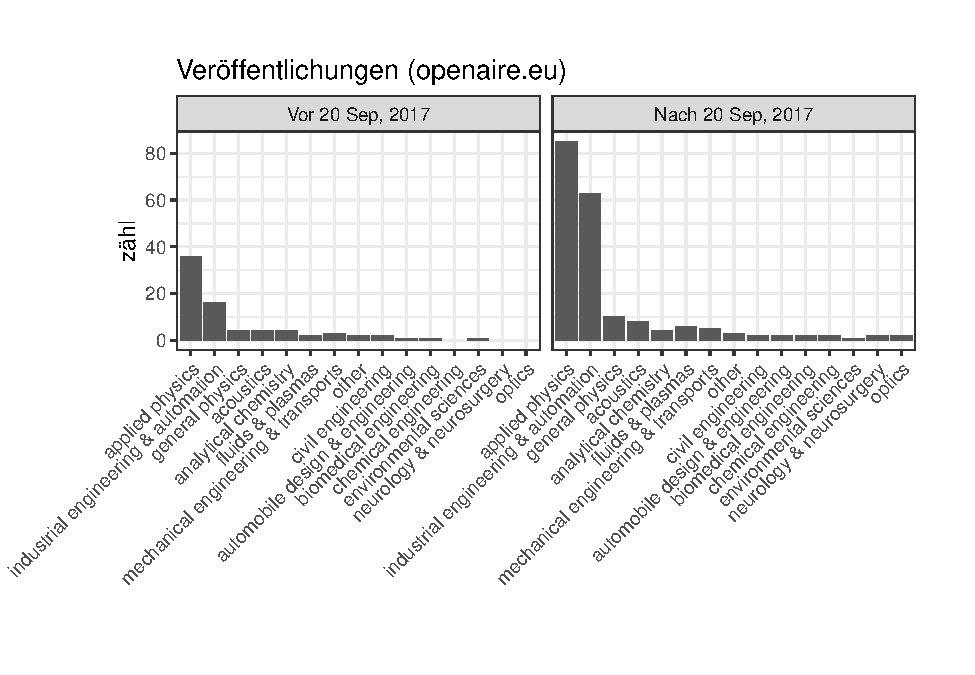
\includegraphics{_main_files/figure-latex/plot-1.pdf}
\caption{\label{fig:plot}Veröffentlichungen nach (Teil-)Disziplinen kategorisiert und in zwei Gruppen aufgeteilt: Vor 20 Sep, 2017 und Nach 20 Sep, 2017.}
\end{figure}

Anwendungen in Medizin und Naturwissenschaften legen nahe, dass zukünftige Entwicklungen von Linearmotoren eine weitere Optimierung der Präzision (im Mikro- bis Nanometerbereich) sowie eine weitere Reduzierung von Größe und Gewicht dieser Geräte umfassen werden. Eine genauere Untersuchung der von der OpenAire-Plattform gewonnenen Daten (Abb. \ref{fig:plot}) zeigt, dass weitere Verbesserungen durch die Aufnahme von Störeffekten wie Reibung, Drehmomenten und anderen parasitären Kräften erzielt werden können. Diese aktive Forschungsdisziplin der Linearmotor-Präzisionsoptimierung lässt sich grob in drei Ansätze unterteilen. Das erste Lösungspaket umfasst die Untersuchung neuer Rohstoffe, wie z. B. Hybridmaterialien für Eisenkern-Linearmotoren \citep{Liu2021} und Hochtemperatur-Supraleitermagnete für einen energieeffizienteren Stromverbrauch \citep{zhang2016, palka2021}. Das Erfordernis von Seltenerdelementen in diesen Lösungen schränkt die vollständige Implementierung angesichts der Knappheit dieser Ressourcen ein \citep{deboer2013}. Motoren in molekularer Größe, die aus Kohlenstoffnanoröhren bestehen, die durch thermische Gradienten angetrieben werden, und Supraleiter auf Graphenbasis könnten zukünftige Wege zur Größenreduzierung und Energieeffizienz sein, aber diese Materialien sind noch weitgehend experimentell \citep{zambrano2009, cao2018}. Eine zweite Reihe von Lösungen konzentriert sich auf die Verbesserung der Designparameter des Geräts \citep{kuang2017, kramer2021}, während ein dritter Ansatz darauf abzielt, Algorithmen zu verbessern, die Linearmotoren führen, wodurch die Bahnverfolgung verbessert und die Auswirkungen anomaler Kräfte auf die Präzision verringert werden \citep{nguyen2016, mo2017, yunbo2018, chen2020, yao2021}.

\hypertarget{optim}{%
\section{Optimierungspotentiale}\label{optim}}

Das Gewicht der Eisenkernläufer führt aufgrund der erhöhten Trägheit des Systems zu höheren Energiekosten. Im Gegensatz dazu wurden eisenlose Linearmotoren entwickelt, um diese höhere Trägheitsbelastung zu überwinden, indem leichtere Materialien in der Kraft verwendet werden. Bei letzterer Konstruktion sind die Spulen der Kraft in Epoxidharz gegossen. Dies hat einige offensichtliche Vorteile in Bezug auf das Gewicht des Läufer, was zu einer höheren Beschleunigung und Verzögerung von Bewegungen führt. Dennoch haben eisenlose Linearmotoren einige Einschränkungen im Vergleich zur eisenbehafteten Variante, was hauptsächlich zu höheren Nennkräften für ähnlich große eisenlose Varianten führt. Um ähnliche Spezifikationen zu erreichen, müssen einige Einschränkungen des eisenlosen Linearmotors überwunden werden. Diese Einschränkungen lassen sich grob in drei Gruppen einteilen:

\textbf{Materialien}
Die Epoxidharz-Läufer von eisenlosen Linearmotoren haben eine geringere Wärmeleitfähigkeit und Struktursteifigkeit als die Variante mit Eisenkern. Dies kann überwunden werden durch:

\begin{itemize}
\tightlist
\item
  Entwicklung besser wärmeleitfähiger Epoxidharze. Dies kann möglicherweise durch die Verwendung von Nanopartikeleinschlüssen erreicht werden, die in das Epoxidharz eingebettet sind \citep{fu2010}.
\item
  Verbesserung der strukturellen Steifheit des Epoxidharzes. Kunststoffe mit einer hohen strukturellen Steifigkeit sind ein Forschungsschwerpunkt in prothetischen Studien. Diese Fortschritte in der Prothetik könnten möglicherweise in eisenlose Forcer-Designs implementiert werden.
\item
  Verringerung des Gewichts der Spule durch Verwendung von (Hochtemperatur-)supraleitenden Spulen mit geringerem Energieverbrauch \citep{palka2021}. Noch spekulativer ist die Umsetzung von noch weitgehend theoretischen Supraleitern wie „Magic-Winkel-Graphen`` \citep{cao2018}.
\end{itemize}

\textbf{Design optimization}\\
The Y-beam design is an example of a geometric configuration that improved the efficiency of ironless linear motors. Building on this progresses in forcer design one can:

\begin{itemize}
\tightlist
\item
  further improvement motor geometry and other design parameters by state-of-the-art topological and magnetic flux models {[}e.g., duan2011{]}.
\item
  adopt precision manufacturing processes (such as laser metal cutting) to actually implement design improvements with minimal amounts of variation. Minimization of production errors will increase the efficiency of these systems in real-world applications.
\end{itemize}

\textbf{Adaptive algorithms}\\
Computational routines for movement tracking and corrective feedback will help overcome magnetic flux interaction and other parasitic forces that negatively influence the machine's performance \citep{nguyen2016}. Such algorithms can benefit from:
re
- increased computational power that matches the speed of movement in the mechanical system. This will benefit the overall performance.
- implementing self-supervised machine algorithms that can iteratively learn the best routine for certain movements within a specific system.

Improvements in all of these categories can improve the system's performance without the need of larger and heavier forcers. Reversely, this also creates opportunities to further reduce the size and weight of linear motors. This would be beneficial for the high precision applications, such as, biomedical devices, surgical tools and high-end optics, that require nano- to micro-scale spatial precision with a very consistent velocity control of movement.

\hypertarget{consortium}{%
\section{Consortium}\label{consortium}}

Based on the observations in section \ref{optim} there seem to be a high potential for improving the precision of ironless linear motors. These specific devices have numerous high precision applications. Hence I framed the goal of the consortium around a specific real world use case. In this consortium I envision ironless linear motor design optimization as a potentially highly rewarding endeavour to improve linear motor performance in exoskeletons (for neuromuscular disorders and rehabilitation) and prosthetics (internal and external). The proposed solutions could improve the precision of mechanic movements to more closely mimic the human motor system, result in more durable and low-weight devices that benefit the comfort of the user, and extends the battery lifetime. These features have been identified as bottlenecks in exoskeletons and prosthetics development \citep{pasquina2015}. I divided the roles of the consortium members as follows: ``material development'', ``design optimization'', and ``testing and production''. For each of these roles I listed a number of research institutes and companies that will realise the above mentioned specifications for linear motor optimization.

\hypertarget{material-development}{%
\subsection{Material development}\label{material-development}}

Developing material with greater heat conductivity and structural stiffness is a critical aspect that could advance the linear moto design by increasing the precision of movements and the durability of the forcer.

\begin{itemize}
\tightlist
\item
  \href{https://www.ipfdd.de/en/research/institute-of-macromolecular-chemistry/functional-nanocomposites-and-blends/fields-of-research/composites-containing-carbon-nano-structures/}{Leibniz-Institut für Polymerforschung}, Dresden: This institute has a research group especially dedicated to researching the effect of carbon nanostructure inclusion in polymers on thermal properties. This expertise would be suited to develop epoxyresins for ironless forcers with better heat conducting properties.
\end{itemize}

\hypertarget{design-optimization}{%
\subsection{Design optimization}\label{design-optimization}}

The proposed consortium will combine state-of-the-art artificial neural networks to optimize design parameters before the actual production starts. Artificial neural networks have been proven particularly useful to model non-linear systems and have been successfully applied in topology optimization and heat conduction system design problems \citep{zhang2021}.

\begin{itemize}
\item
  \href{https://www.iais.fraunhofer.de/}{Fraunhofer-Institut für Intelligente Analyse- und Informationssysteme}, Dresden: Has a long history of researching intelligent digital solutions and subsequently applying this knowledge to real world problems. In addition, the institute has an extensive network that contains educational institutes, start-ups and cooperations, which could supplement the consortium.
\item
  \href{https://www.celus.io/}{CELUS GmbH}, München: Is an AI-powered start-up that focusses on electronics engineering processes, including: smart solutions for material selection and digital twins of electronic components. There experience could help facilitate the design phase but also construct adaptive feedback algorithms that help regulate movement and compensate for unwanted disruptive forces (e.g.~magnetic flux interaction and parasitic forces).
\end{itemize}

\hypertarget{testing-and-production}{%
\subsection{Testing and Production}\label{testing-and-production}}

It is important to have a production line that can deliver the same level of accuracy as the parameters used in the design phase. The prerequisites for such a level of accuracy encompasses precision manufacturing and critical quality checks along the production line. This allows real life testing of the devices in experimental set-ups and enables a comparison with the model output of the design phase. Trial experiments are, furthermore, required to test the user's satisfaction with the newly developed devices.

\begin{itemize}
\item
  \href{https://www.faulhaber.com/en/markets/medical/exoskeletons-prosthetics/}{Faulhaber Gruppe}, Schönaich: Is a manufacturer of high-tech miniature and micro motors, among which linear motors, and they actively research solutions for the prosthetics and exoskeleton market. The decades of experience in micro-electronic production, and the level of accuracy in their production lines, will realise the design goals as set-out in the design phase.
\item
  \href{https://www.ottobock.com/de-de/startseite}{Ottobock SE \& Co.~KGaA}, Duderstadt: This firm resides at the end of the production chain for prosthetics and exoskeleton products. This company regularly performs clinical trials of their products to quantify performance and user satisfaction. The outcomes of these trails can, in tuen, feed back important information into the design face, thereby closing the circle of this research and development process.
\end{itemize}

\hypertarget{zeitplan}{%
\section{Zeitplan}\label{zeitplan}}

  \bibliography{book.bib,packages.bib,linearmotors.bib}

\end{document}
